
\documentclass{article}

%% Packages for French writing
\usepackage[francais]{babel}
\usepackage[utf8]{inputenc}
\usepackage[T1]{fontenc}
\usepackage{layout}

%% Packages for Math symbols
\usepackage[fleqn]{amsmath}
\usepackage{amssymb}
\usepackage{mathrsfs}

%% Packages for figures insertion
\usepackage{graphicx}
\usepackage{wrapfig}
\usepackage{framed}
\usepackage{float}

%% Package for document margin editing
\usepackage[top=2cm, bottom=2cm, left=2cm, right=2cm]{geometry}

%% Package for source code insertion
\usepackage{listings}
\usepackage{xcolor}
\definecolor{grey}{rgb}{0.97, 0.97, 0.97}
\definecolor{darkred}{rgb}{0.42, 0, 0}
\definecolor{darkblue}{rgb}{0, 0, 0.42}
\definecolor{darkgrey}{rgb}{0.22, 0.22, 0.82}
\definecolor{green}{HTML}{088A08}
\lstset{
  basicstyle=\small\sffamily\footnotesize,
  captionpos=b,
  numbers=left,
  numberstyle=\tiny,
  tabsize=4,
  frame=trBL,
  backgroundcolor=\color{grey},
  commentstyle=\color{green},
  keywordstyle=\color{darkblue}\bf,
  identifierstyle=\color{darkgrey},
  stringstyle=\color{darkred}
}

\setlength\parindent{0pt}
\setlength\parskip{3pt}
\title{Rapport de projet VLSI}
\author{Nicolas Phan, Kevin Mambu}
\date{pour le 26 Janvier 2018}
\begin{document}
\pagestyle{headings}
\maketitle
\tableofcontents
\newpage

%==================================================================================================
%=========================  Introduction  =========================================================
%==================================================================================================
\section{Introduction}

%----------------- Objectif -----------------------------------------------------------------------
\subsection{Objectif}

Le but de notre projet est de concevoir un processeur ARM, c'est à dire un processeur conforme
à l'architecture décrite dans la documentation ARM donnée en cahier des charges.

%----------------- Processus de developpement -----------------------------------------------------
\subsection{Processus de développement}

La conception de ce processeur se fera en quatre grandes étapes :

\begin{figure}[ht]
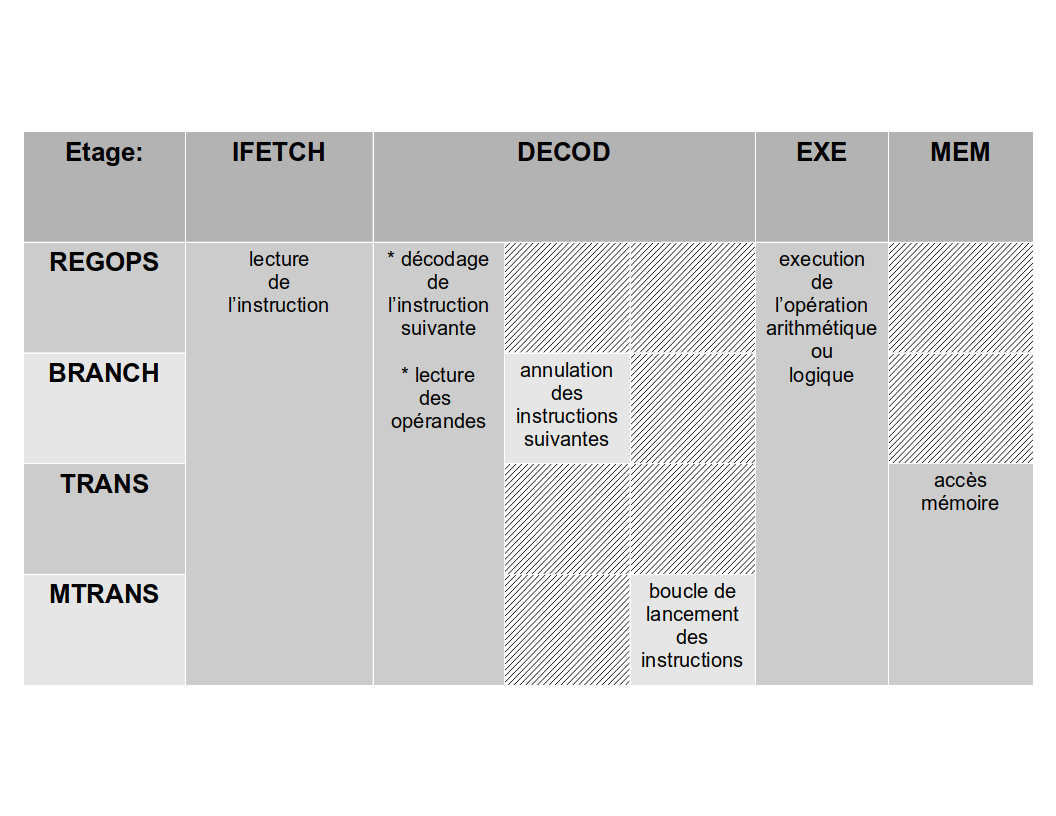
\includegraphics[width=0.75\textwidth]{pics/blank.png}
\centering
\caption{Schema-bloc des étapes de conception du processeur} 
\end{figure}

\begin{enumerate}
\item \textbf{Modélisation}  : Cela consiste en la description d'un modèle du processeur,
                      la description peut avoir différents niveaux d'abstraction
                      du plus abstrait (description du comportement du circuit seulement)
                      au plus concret (schema des portes logiques du circuit)
                      \textit{Nous utiliserons le langage VHDL pour décrire notre modèle de processeur}
\item \textbf{Simulation}    : Il s'agit de simuler notre processeur.
                      \textit{Nous utiliserons le simulateur ghdl ainsi que des bancs de tests VHDL
                      et une plateforme de simulation d'exécution de programmes ASM et C}
\item \textbf{Placement, Routage} : Dans cette étape, nous passons d'un modèle VHDL du circuit à un
                          dessin du masque de notre processeur, prêt à être envoyé en fonderie.
                          \textit{Nous utiliserons les outils druc, cougar, lvx, tas et s2r pour cela}
\item \textbf{Fonderie} :          Cette étape est réalisée par un fondeur tiers.
\end{enumerate}

%==================================================================================================
%=========================  Modelisation  =========================================================
%==================================================================================================
\section{Modélisation}

\subsection{Design général du processeur}

Le processeur doit pouvoir exécuter toutes les instruction du jeu ARM avec le moins
de matériel possible, de plus, nous devrons concevoir un processeur pipeliné asynchrone.
La figure \ref{etages} illustre le découpage en étages de notre pipeline avec les opérations effectuées
par chaque étage pour chaque type d'instruction.
Les types d'instructions que nous étudierons seront les instructions de data processing (regops),
les instructions de branchement (branch), les transferts mémoires simples (trans) et multiples (mtrans).

\begin{figure}[ht]
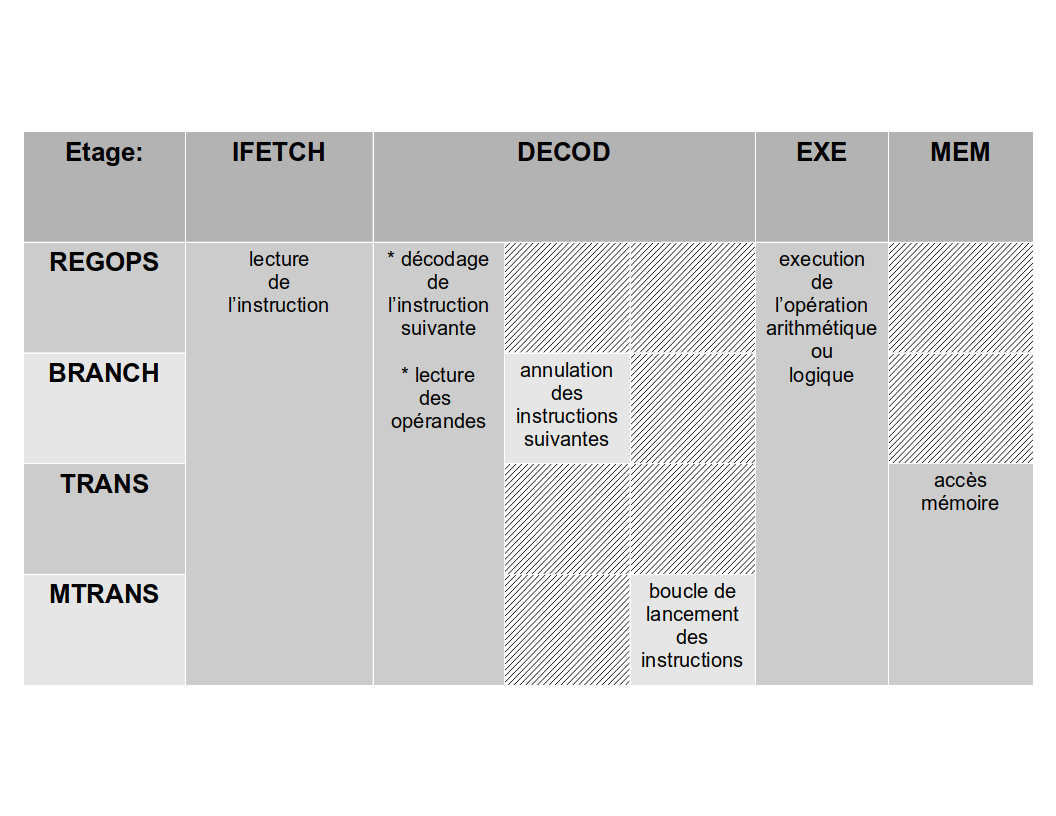
\includegraphics[scale=1]{pics/blank.png}
\centering
\caption{Découpage en étages du processeur}
\label{etages}
\end{figure}

\subsection{Modélisation de l'étage EXE}

\par
C'est à l'étage EXE que se feront les opérations de calcul lors de l'execution d'instructions,
cela comprend le calcul de l'adresse destination lors d'un branchement.
Pour concevoir cet étage, nous devons nous demander quelles sont tous les calculs possibles
que l'étage devra pouvoir réaliser.

\par
Les différents types d'instructions que nous avons sont les regops, les branch, les trans et mtrans,
or les branch, trans et mtrans n'ont besoin d'effectuer que des additions (pour le calcul d'adresses
mémoire) et les regops contiennent une instruction d'addition, donc si l'étage EXE peut effectuer
les calculs nécéssaires aux regops, a fortiori il couvre aussi les branch et transferts mémoire.
Cela réduit le problème au cas des regops.

\par
Il faut lister l'ensemble des calculs que EXE devra effectuer et les réécrire
de manière standardisée pour les décomposer en un sous-ensemble de calculs élémentaires.
Cela nous permettra de trouver une implémentation de EXE réduisant au maximum le matériel nécéssaire.

\begin{table}[H]
\centering
\begingroup
\setlength{\tabcolsep}{5pt}
\renewcommand{\arraystretch}{1.1}
\begin{tabular}{ | c | c | c | }
\hline
Instruction & Calcul demandé & Calcul standardisé  \\
\hline
\tt{AND}      & \tt{ op1 AND op2 }                 & \tt{ op1 AND op2 } \\
\hline
\tt{EOR}      & \tt{ op1 XOR op2 }                 & \tt{ op1 XOR op2 }       \\
\hline
\tt{SUB}      & \tt{ op1 - op2 }                   & \tt{ op1 + $\overline{\tt{op2}}$ + 1 }       \\
\hline
\tt{RSB}      & \tt{ op2 - op1 }                   & \tt{ op1 + op2 }       \\
\hline
\tt{ADD}      & \tt{ op1 + op2 }                   & \tt{ op1 + op2 }       \\
\hline
\tt{ADC}      & \tt{ op1 + op2 + c }               & \tt{ op1 + op2 }       \\
\hline
\tt{SBC}      & \tt{ op1 - op2 + c - 1 }           & \tt{ op1 + op2 }       \\
\hline
\tt{RSC}      & \tt{ op2 - op1 + c - 1 }           & \tt{ op1 + op2 }       \\
\hline
\tt{TST}      & \tt{ op1 AND op2 }                 & \tt{ op1 + op2 }       \\
\hline
\tt{TEQ}      & \tt{ op1 XOR op2 }                 & \tt{ op1 + op2 }       \\
\hline
\tt{CMP}      & \tt{ op1 SUB op2 }                 & \tt{ op1 + op2 }       \\
\hline
\tt{CMN}      & \tt{ op1 ADD op2 }                 & \tt{ op1 + op2 }       \\
\hline
\tt{ORR}      & \tt{ op1 OR op2 }                  & \tt{ op1 + op2 }       \\
\hline
\tt{MOR}      & \tt{ op2 }                         & \tt{ op1 + op2 }       \\
\hline
\tt{BIC}      & \tt{ op1 AND NOT op2 }             & \tt{ op1 + op2 }       \\
\hline
\tt{MVN}      & \tt{ NOT op2 }                     & \tt{ op1 + op2 }       \\
\hline
\end{tabular}
\endgroup
\caption{Standardisation des calculs demandés par les regops}
\label{standard}
\end{table}

On peut voir sur la Table \ref{standard} que l'ensemble des calculs demandés se décompose
en calculs élémentaires suivants :
\begin{itemize}
  \item ADD, AND, OR, XOR
  \item Inversion des entrées au préalable
  \item Ajout d'un 1 pour l'addition (retenue en entrée)
\end{itemize}

De plus, le jeu d'instruction ARM spécife que l'opérande 1 peut subir un décalage
parmi 5 types (lsl, lsr, asr, ror, rrx) et qu'à chaque opération, les flags de sortie
doivent être calculés, on a donc :
\begin{itemize}
  \item Décalage de l'opérande 1
  \item Calcul des flags de sortie
\end{itemize}

Avec tous ces éléments, nous aboutissons au schema Figure \ref{exe} pour EXE.

\begin{figure}[ht]
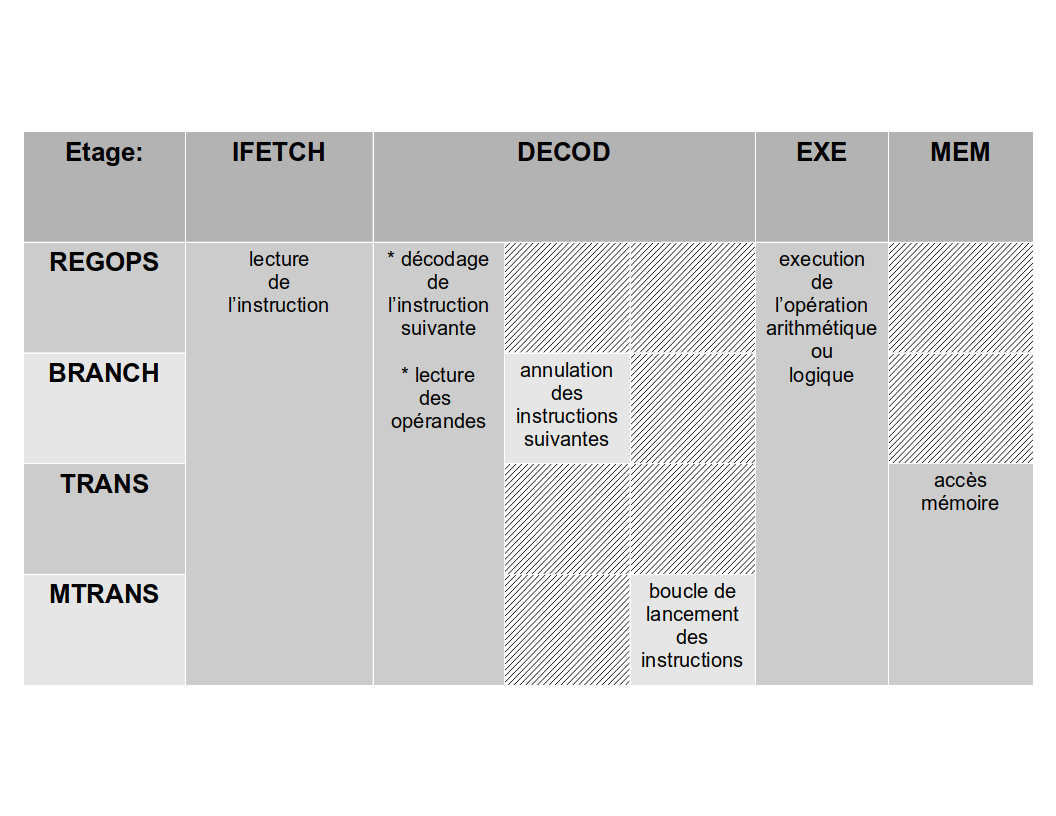
\includegraphics[scale=1]{pics/blank.png}
\centering
\caption{Schema de l'étage EXE}
\label{exe}
\end{figure}

\subsubsection{Modélisation de l'ALU}

L'ALU doit pouvoir effectuer les opérations ADD, AND, OR et XOR sur deux entrées de 32bits,
et pour l'addition elle doit pouvoir prendre en compte une retenue en entrée et en sortie.

Notre implémentation est celle en Figure \ref{alu} : L'ALU effectue de toutes manières les
4 opérations sur ses entrées, mais ne prend que le résultat de l'opération qui nous intéresse.

Pour le calcul des flags, le bloc "=0" effectue un simple AND entre tous les bits du résultat,
le bloc "<0" vérifie si le MSB est égal à 1, on remarque que par la manière dont est construit
le système de nombres signés, la condition "<0" est très simple à vérifier. Puis pour le bloc "overflow",
on prend le 33ème bit du résultat de l'addition, il y a overflow s'il n'est pas nul (le résultat va au-delà
du range des 32 bits).

\begin{figure}[ht]
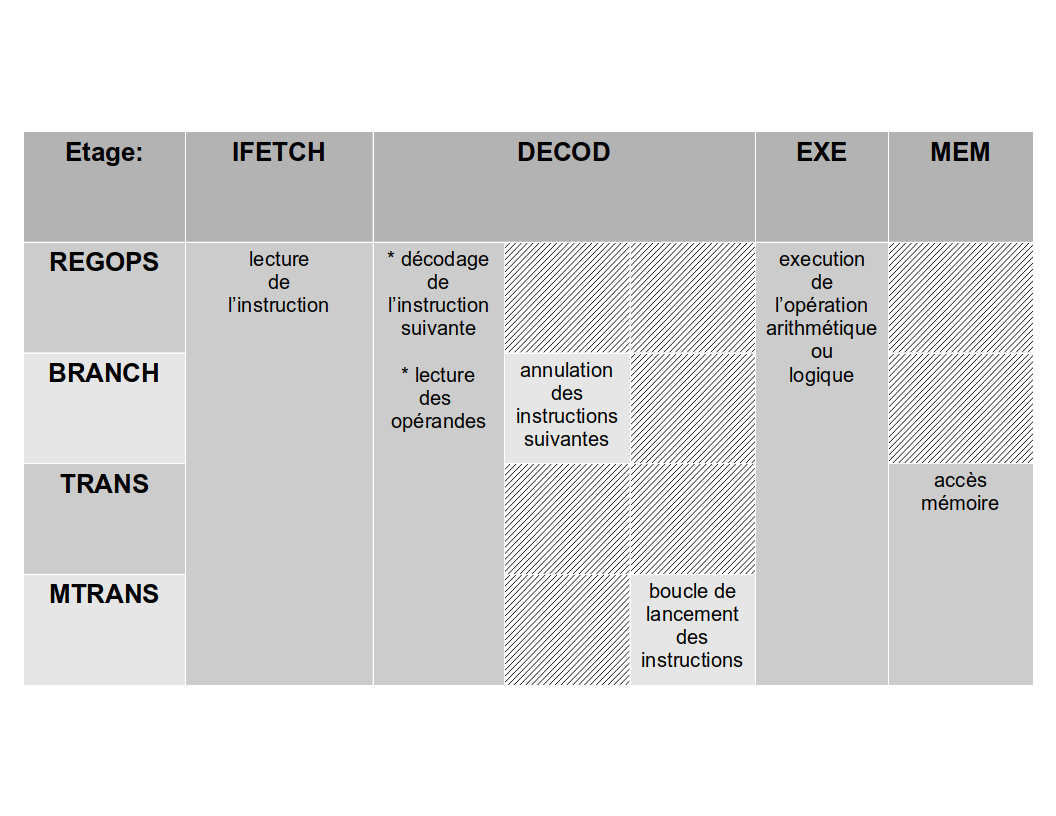
\includegraphics[scale=1]{pics/blank.png}
\centering
\caption{Schema de l'ALU}
\label{alu}
\end{figure}

\subsubsection{Modélisation du Shifter}

\begin{figure}[H]
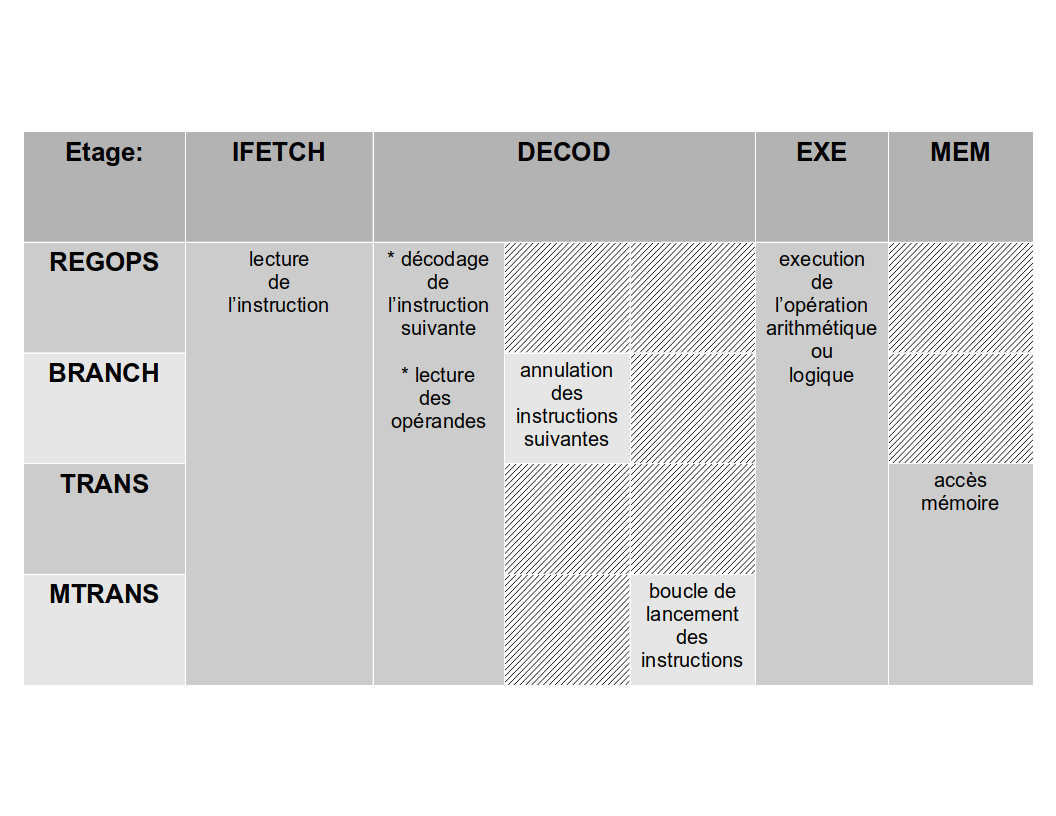
\includegraphics[scale=1]{pics/blank.png}
\centering
\caption{Schema du Shifter}
\label{shifter}
\end{figure}

Tout comme l'ALU peut effectuer différentes opérations, le shifter peut effectuer différents
types de décalages (LSL, LSR, ASR, ROR, RRX) donc de la même manière, notre implémentation
du shifter en Figure \ref{shifter} effectue tous les types de décalages possibles et choisit
le résultat qui nous intéresse.

\begin{figure}[ht]
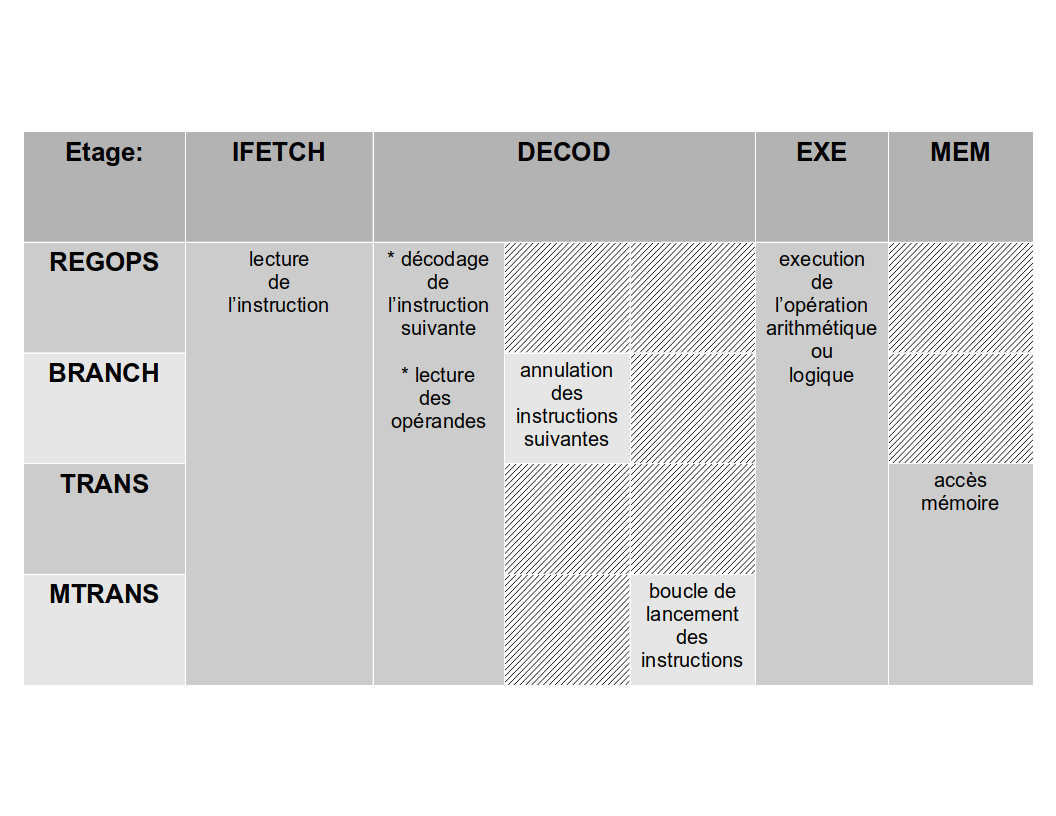
\includegraphics[scale=1]{pics/blank.png}
\centering
\caption{Schema de la partie LSL du Shifter}
\label{shifter_lsl}
\end{figure}

Ensuite pour réaliser l'opération LSL, en Figure \ref{shifter_lsl},
on observe chaque bit du \texttt{shift\_value} :
si le bit $n$ est à \texttt{1}, alors l'opérande subit un décalage de $2^n$.
Le décalage total subi par l'opérande source est donc de :

\begin{eqnarray*}
  \sum_{\substack{k \in [[0, 31]] \\ \texttt{shift\_value(k)} = 1}} 2^k &= \texttt{shift\_value}
\end{eqnarray*}

La même logique est utilisée pour implémenter les autres types de décalages.

\subsubsection{Ajouts sur EXE}

\textbf{Le flag C}
D'après la doc ARM, le flag C en sortie d'une opération peut être la retenur en sortie d'addition
pour les opérations arithmétiques ou en sortie de shift pour les opérations logiques.
Puis pour savoir si l'opération en cours est arithmérique ou logique, il suffit de voir si
l'ALU réalise une addition ou autre chose.

La pre/post indexation
Lors d'un accès mémoire, le jeu ARM offre la possibilité de choisisr si l'adresse prise en compte
pour un accès mémoire est l'adresse de base ou l'addresse base + offset.
Dans EXE, cela équivaut à choisir entre l'opérande 2 et le résultat en sortie d'ALU,
cela mène au schema en Figure \ref{exe2}.

\begin{figure}[ht]
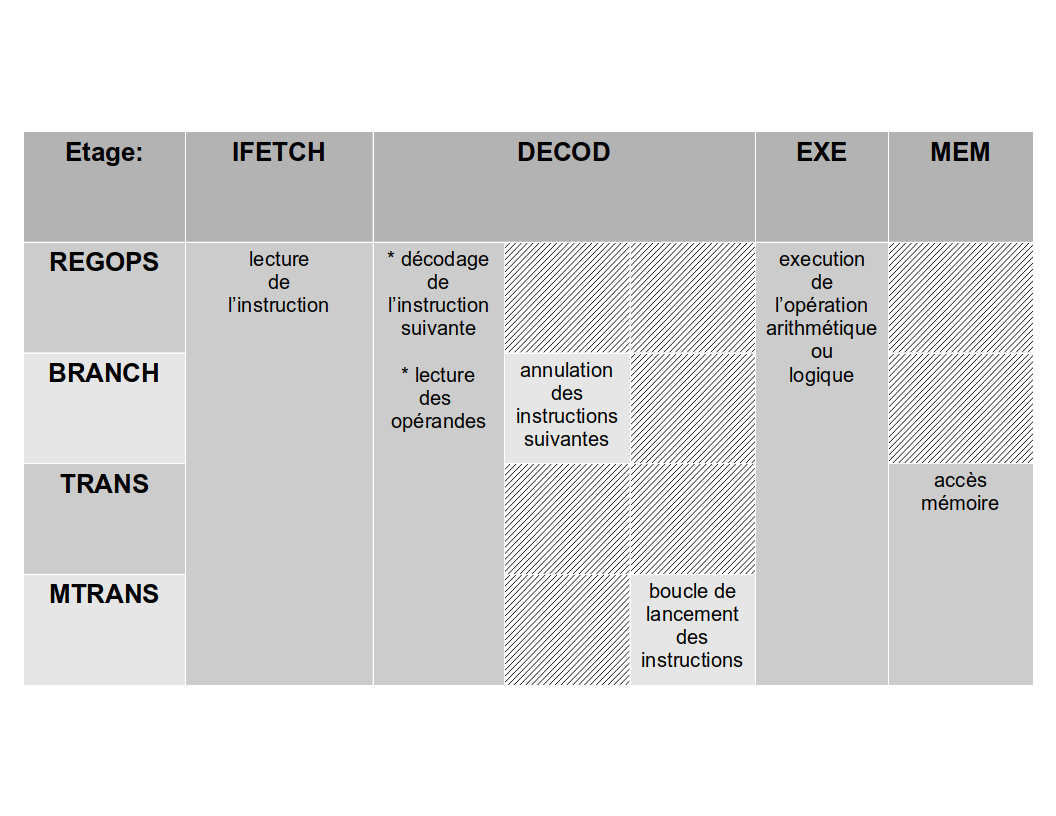
\includegraphics[scale=1]{pics/blank.png}
\centering
\caption{Schema amélioré de EXE}
\label{exe2}
\end{figure}


%==================================================================================================
%=========================  End of the Document  ==================================================
%==================================================================================================

\end{document}
